\documentclass{article}
\usepackage{graphicx}
\usepackage[margin=1.5cm]{geometry}
\usepackage{amsmath}

\begin{document}

\title{Wednesday Reading Assessment: Unit 8, Momentum}
\author{Prof. Jordan C. Hanson}

\maketitle

\section{Memory Bank}

\begin{itemize}
\item $\vec{p} = m\vec{v}$ ... Definition of momentum.
\item $\vec{p}_{\rm total} = \vec{p}_1 + \vec{p}_2$ ... Total momentum is the sum of two momenta.
\item $\vec{p}_{\rm total,i} = \vec{p}_{\rm total,f}$ ... Momentum is conserved, like energy.
\end{itemize}

\section{Momentum}

\begin{enumerate}
\item
\begin{figure}[ht]
\centering
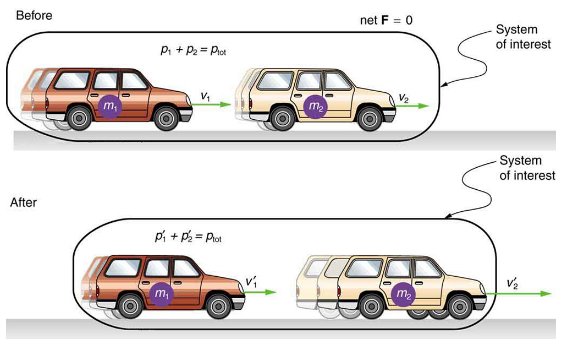
\includegraphics[width=0.5\textwidth]{cars.png}
\caption{\label{fig:cars} One car bumps another.}
\end{figure}
Suppose a hapless Whittier student is on their commute to class one morning when they are bumped by the car behind them (See Fig. \ref{fig:cars}).  Suppose $m_1 = 2000$ kg, and $m_2 = 1400$ kg.  (a) If the initial velocity of the car with $m_1$ is 4 m/s, what is its initial momentum? (b) If the initial velocity of the Whittier student's car with mass $m_2$ is 0 m/s, what is its initial momentum? (c) What is the total initial momentum? (d) If the final speed of the car with $m_1$ is 0 m/s, what is the final speed of the Whittier student's car with $m_2$ ? \\ \vspace{2cm}
\item In the above problem, is the initial total kinetic energy the same as the final total kinetic energy?  Why or why not?
\end{enumerate}
\end{document}
